\subsection{Baroclinic eddies}

% TODO: mention \Delta z

The previous two test cases were only two-dimensional, and therefore couldn't incorporate the influence of the Coriolis force. We now introduce a test case that involves a baroclinically unstable temperature front in a periodic channel with rotation. This test case was presented by \citet{ilicak12}, as the baroclinically unstable front quickly leads to vigorous eddying without either mechanical or buoyancy forcing, thus it is a closed system suitable for analysis by changes in RPE. The domain is a periodic channel in the x direction, \SI{160}{\kilo\metre} wide by \SI{500}{\kilo\metre} long, with a depth of \SI{1000}{\metre} (\cref{fig:eddies-snapshot_ic}). The front has a sinusoidal initial meridional position, defined as

\begin{equation}
  y_w(x) = y_0 - y_A \sin\left(2\pi k \frac{x}{L_x}\right),
\end{equation}

where $y_A = \SI{40}{\kilo\metre}$ is the amplitude, $y_0 = \SI{250}{\kilo\metre}$ is the centre of the domain, $k = 3$ and $L_x = \SI{160}{\kilo\metre}$ ensure that three wavelengths span the width of the domain. The initial temperature distribution in the domain is given by

\begin{equation}
  \Theta(x,y,z) = \begin{cases}
    \Theta_0(z) & y \ge y_w(x) + \Delta y, \\
    \Theta_0(z) - \Delta \Theta \left(1 - \frac{y - y_w(x)}{\Delta y}\right) & y_w < y < y_w + \Delta y, \\
    \Theta_0(z) - \Delta \Theta & y \le y_w(x),
  \end{cases}
\end{equation}

where $\Theta_0(z)$ is a linearly stratified background between \SI{10.1}{\celsius} and \SI{13.1}{\celsius}, $\Delta y = \SI{40}{\kilo\metre}$ is the width of the front and $\Delta \Theta = \SI{1.2}{\celsius}$ is the temperature difference across the front. Additionally, a temperature perturbation is added to the crest of one of the waves to promote instability. The region over which the perturbation is added is bounded by $x_2 \le x \le x_3$ and $y'_w - \Delta y / 2 \le y \le y'_w + \Delta y / 2$, where

\begin{equation}
  y'_w(x) = y_0 - \frac{y_A}{2}\sin\left(\pi \frac{x - x_2}{x_3 - x_2}\right).
\end{equation}

\begin{figure}
  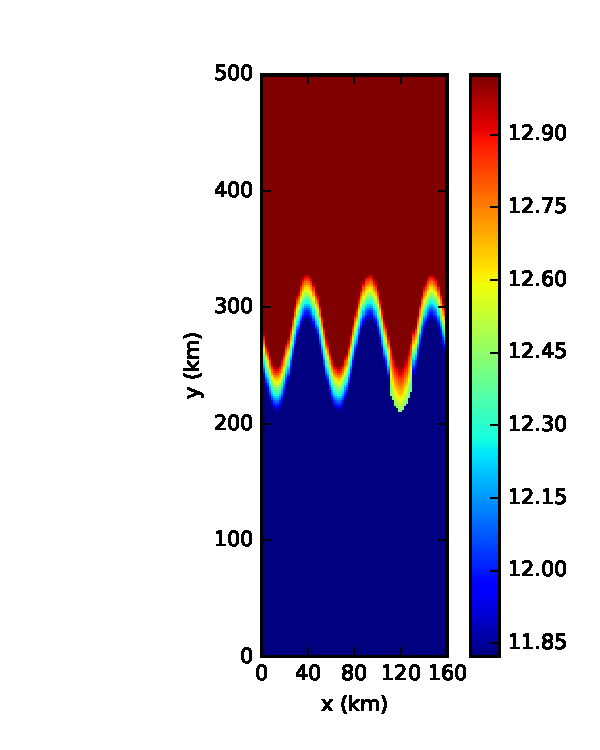
\includegraphics{../plots/eddies_snapshot_dx1_initial.pdf}
  \caption{\label{fig:eddies-snapshot_ic} Snapshot of initial condition of surface temperature for the baroclinic eddies test case at \SI{1}{\kilo\metre} horizontal resolution. The temperature perturbation can be seen at the third trough in the sinusoidal front.}
\end{figure}

\begin{figure}
  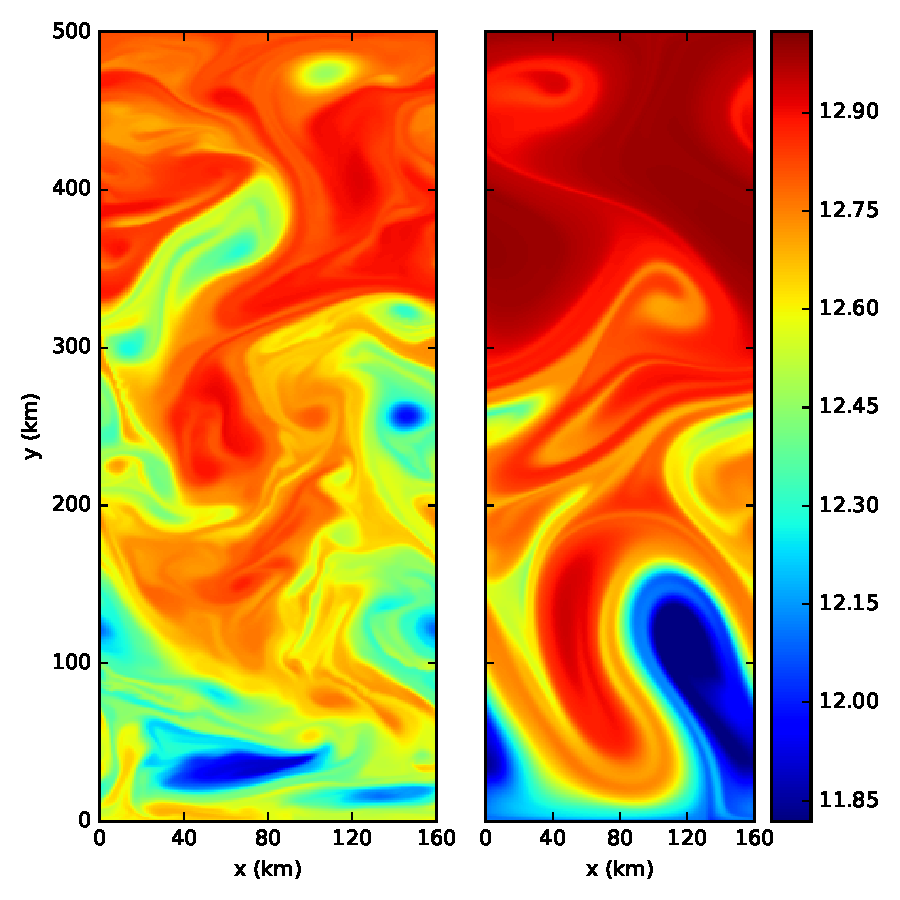
\includegraphics{../plots/eddies_snapshot_dx1.pdf}
  \caption{\label{fig:eddies-snapshot} Snapshots of surface temperature (\si{\celsius}) after 320 days of simulation at \SI{1}{\kilo\metre} horizontal resolution. Left panel is low viscosity (high grid Reynolds number), $\nu_h = \SI{1}{\square\metre\per\second}$. Right panel is high viscosity (low grid Reynolds number), $\nu_h = \SI{200}{\square\metre\per\second}$. There is more mixing at low viscosities, but the features are finer in scale.}
\end{figure}

The perturbation itself is defined by the temperature anomaly

\begin{equation}
  \Theta'(x,y) = \Delta\Theta'\left(1 - \frac{y - y'_w(x)}{\Delta y / 2}\right).
\end{equation}

In order to encourage baroclinicity, a quadratic bottom drag with drag coefficient $C_D = 0.01$ is used. Experiments were performed at horizontal resolutions of \SIlist{1;4;10}{\kilo\metre}. For each choice of horizontal resolution, the horizontal viscosities $\nu_h$ were \SIlist{1;5;10;20;200}{\square\metre\per\second}, giving a range of lateral grid Reynolds numbers from $O(1)$ at the highest viscosity, through to $O(1000)$ for the lowest viscosity.

\Cref{fig:eddies-snapshot} shows the surface temperature after the full 320 days of simulation at 1km horizontal resolution, at the lowest and highest viscosities, \SI{1}{\square\metre\per\second} and \SI{200}{\square\metre\per\second}, respectively. In the low viscosity case, strong spurious mixing has occurred, but finer-scale features are also evident. Conversely, the range of intermediate temperatures is significantly less with a higher horizontal viscosity, but the eddies are much weaker due to the momentum damping by the viscosity.

\begin{figure}
  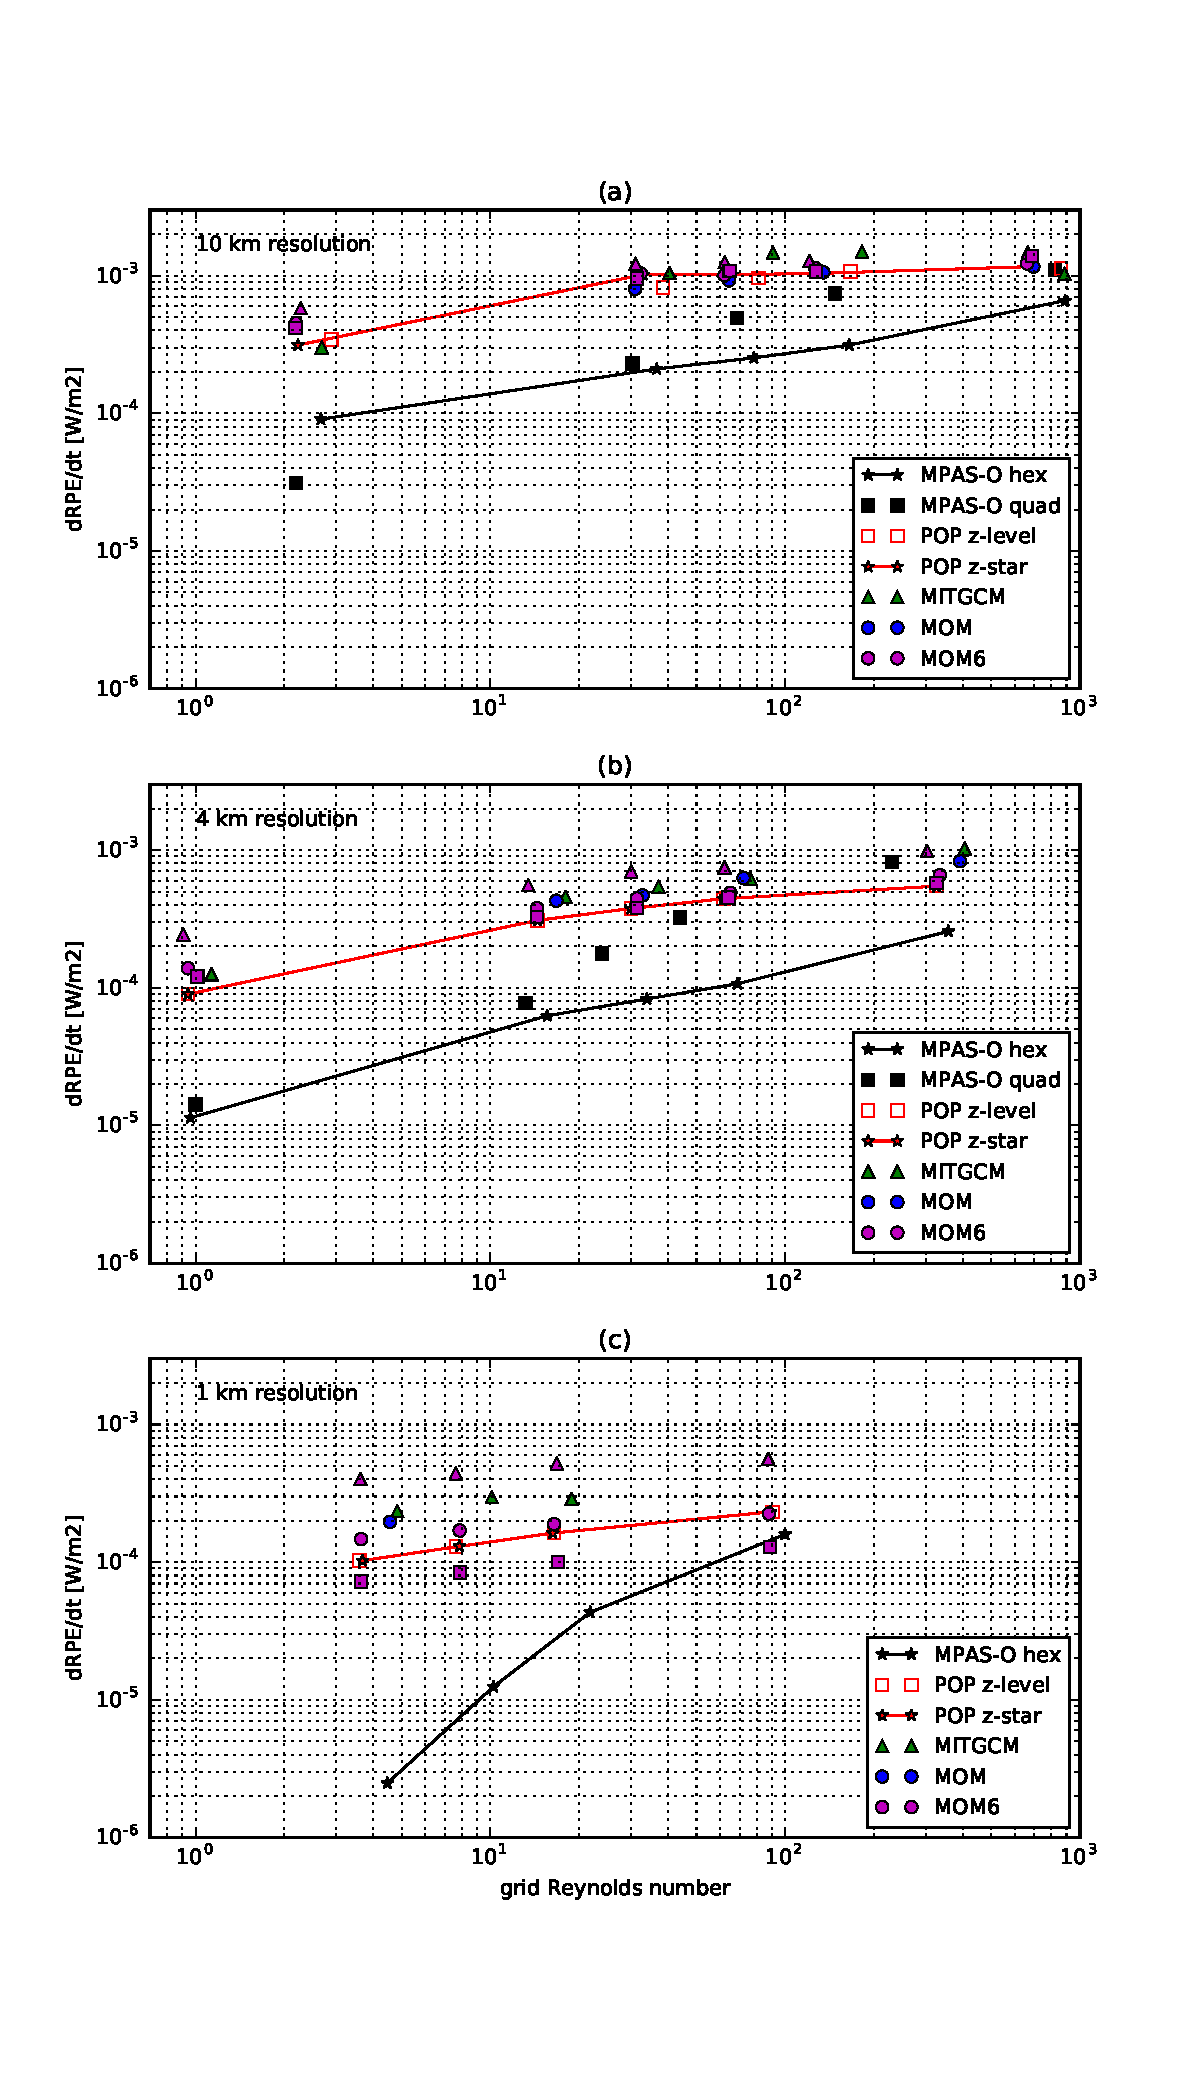
\includegraphics{../plots/eddies_drpe.pdf}
  \caption{\label{fig:eddies-drpe} Rate of RPE change for all experiments. Data from MPAS-O, POP, MITGCM and MOM come from @petersen15 and @ilicak12. MOM6 using the default PLM tracer advection scheme is shown in magenta circles, with the alternate PPM:H3 scheme shown in magenta triangles at \SIlist{10;4}{\kilo\metre} resolution.}
\end{figure}

\Cref{fig:eddies-drpe} shows the rate of RPE change across all tested models for \SIlist{10;4;1}{\kilo\metre} horizontal resolution, respectively. In the 10km experiment, the two available tracer advection schemes were used, PLM shown in magenta circles and the higher-order PPM:H3 scheme in magenta triangles. In the spurious mixing saturation regime of $\mathrm{Re}_\Delta > 10$, MOM6 with the PLM scheme plateaus at a very similar level to MOM and POP. As expected, the PPM:H3 scheme exhibits slightly lower spurious mixing, especially at the lowest grid Reynolds number. However, in the saturation regime the spurious mixing continues to rise slightly with increasing grid Reynolds number, exceeding the PLM scheme.

When the horizontal resolution is decreased to 4km, MOM6 exhibits slightly greater spurious mixing than POP across the range of experiments. At this resolution, the PPM:H3 advection scheme consistently provides a small decrease in spurious mixing as compared to the PLM scheme. However, the improvement in spurious mixing is minor, and may not be worth the extra computational cost involved in invoking the PPM:H3 advection scheme.

\subsubsection{Spurious mixing orientation}

\begin{figure}
  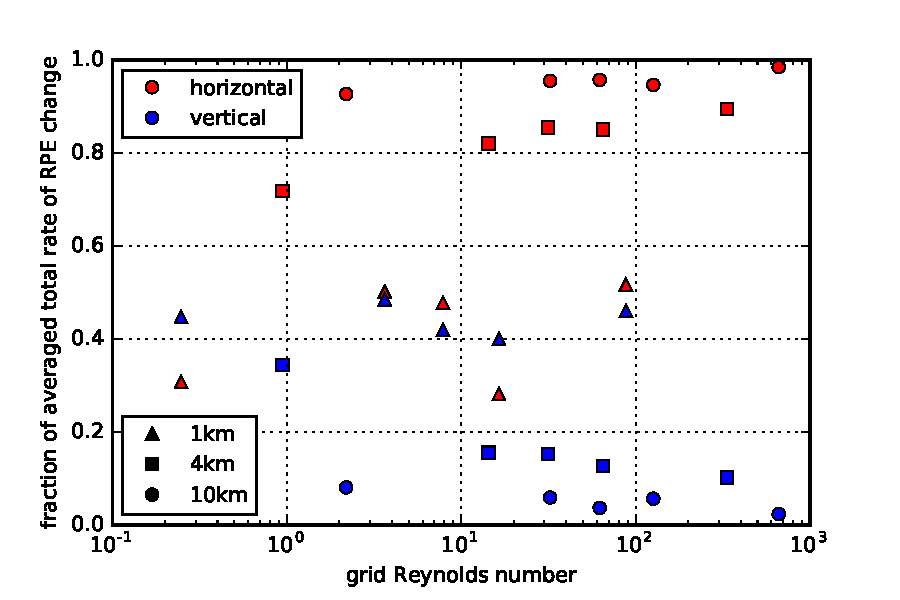
\includegraphics{../plots/eddies_drpe_split.pdf}
  \caption{\label{fig:eddies-drpesplit} Spurious mixing contributions in MOM6 for each horizontal resolution across the range of horizontal viscosities. \SI{1}{\kilo\metre} shown with triangles, \SI{4}{\kilo\metre} with squares and \SI{10}{\kilo\metre} with circles. As resolution increases, the relative contribution of the vertical component also increases, to approximately equal the horizontal component at \SI{1}{\kilo\metre}.}
\end{figure}

- make sure legend is fixed

We consider the orientation of spurious mixing at each of the tested horizontal resolutions in \cref{fig:eddies-drpesplit}. As horizontal resolution increases (grid spacing decreases), the fraction of spurious mixing by regridding/remapping increases. Indeed, at \SI{1}{\kilo\metre} horizontal resolution, horizontal tracer advection and regridding/remapping contribute approximately equally to the total spurious mixing. The reasons for this are likely twofold: firstly, for the same domain size at higher resolution, there are simply more water columns in which regridding/remapping must take place. Secondly, fine-scale features in the flow may cause more interaction between adjacent water columns, or more rapid changes in the Lagrangian vertical grid which require correction by regridding/remapping. This result highlights the importance of further refinement of regridding/remapping schemes and vertical coordinates, particularly as models are run at increasingly higher resolution.

- "anti-spurious mixing"
